\subsection{研究方案和技术路线}

\begin{figure}[h]
    \begin{small}
        \begin{center}
            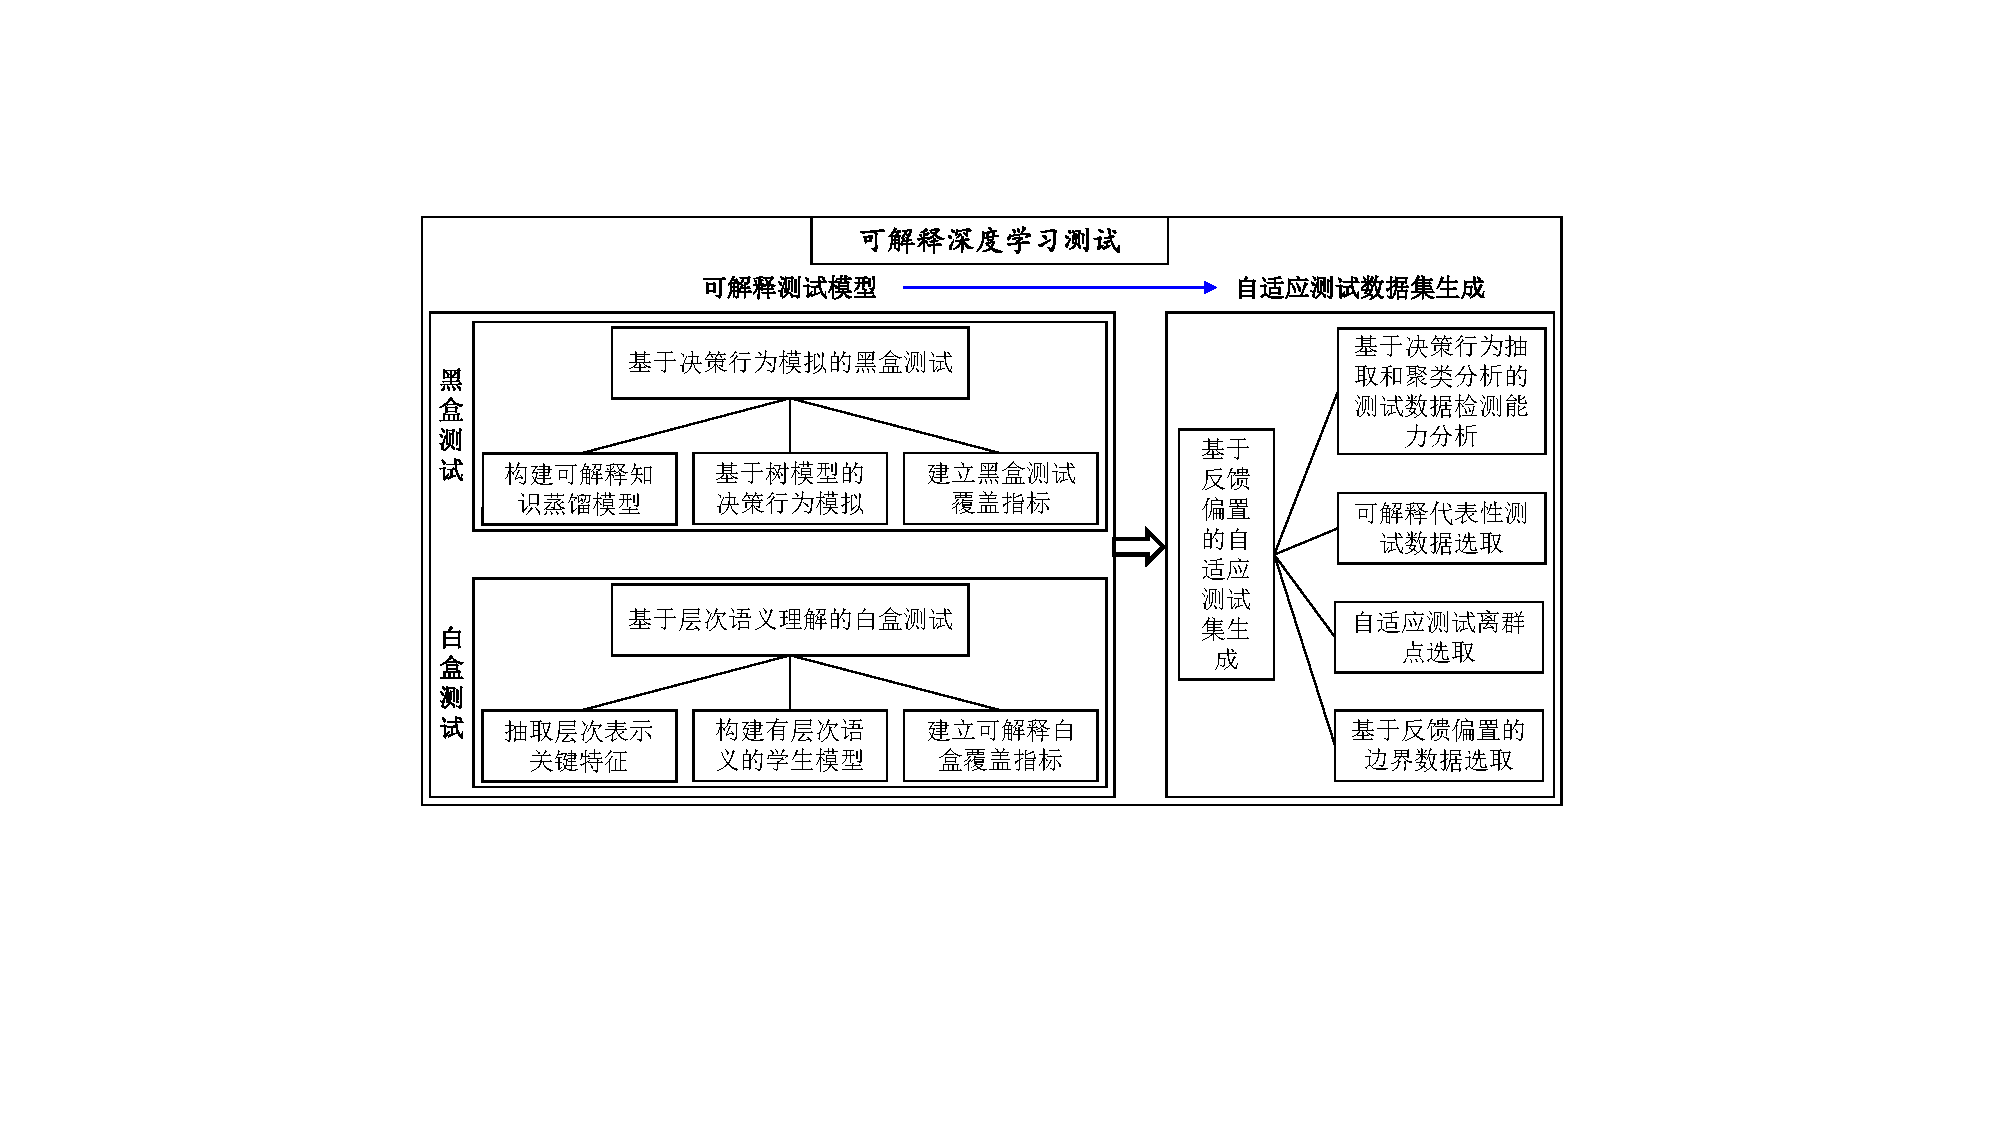
\includegraphics[width=0.95\textwidth]{ch3solution.pdf}
        \end{center}
        \caption{总体技术路线}
        \label{fig:ch3:solution}
    \end{small}
\end{figure}

围绕\ref{ch2content}规划的研究内容和\ref{ch2target}制定的研究目标,本项目拟定的
总体技术路线如\cref{fig:ch3:solution}所示。本项目针对电子医疗记录分析构建基于深
度学习的端到端的解决方案,通过对电子医疗记录数据集依次进行队列识别、EMR插补和可
解释预测,实现对特定患者队列的分析挖掘。本项目的主要研究内容分别对应大数据分析通
用流程中的数据获取、数据预处理和数据分析。此外,鉴于医疗领域的特殊性,本项目的研
究工作需要与医生进行充分的沟通,在模型设计和结果解释等方面融入医生的反馈。下面针
对各部分研究内容,详细介绍其具体研究方案和技术路线。



\subsubsection{基于决策行为模拟的黑盒测试}\label{ch3_1}

\cref{fig:ch3:2Btest}展示了本项目基于决策行为模拟的黑盒测试研究方法,如图所示,
\textbf{本项目拟利用知识蒸馏技术萃取黑盒模型中的知识}。就申请人所知,目前尚未有
基于知识蒸馏的深度学习覆盖度测试研究。首先,本项目利用知识蒸馏技术从黑盒模型(``
教师''模型)中萃取知识,训练一个小模型(``学生''模型)模拟其预测行为,在知识蒸馏
中,``教师''模型被视为黑盒模型,正好契合本项目黑盒测试的场景;其次,本项目拟设计
针对小模型的测试方法,间接评估黑盒模型的泛化能力,一方面,蒸馏得到的``学生''模型
复杂度低,可有效解决深度学习模型测试计算开销大的问题,另一方面,``学生''模型的内
部结构可以自定义,测试者也可访问,本项目拟利用基于树的模型(如:决策树、随机森林
等),以提高测试结果的可解释性。

具体地,给定一个黑盒模型$\mathcal M$,本项目将$\mathcal M$视为``教师''模型,假定
对于任意的输入$x^{(i)}$,测试者仅能得到$\mathcal M$对于该输入预测的概率分布,即
$x^{(i)}$属于各类的概率,记为$p^{(i)}$。$(x^{(i)}, p^{(i)})$的对应关系即为模型
$\mathcal M$中蕴含的知识,将作为训练``学生''模型时的软目标。\textbf{本项目拟构建
基于树的模型作为``学生''模型,记为$\mathcal M_t$,以支持可解释模型测试}。根据知
识蒸馏的思想,在训练``学生''模型时,本项目融合软目标$(x^{(i)}, p^{(i)})$和硬目标
$(x^{(i)}, y^{(i)})$构建``学生''模型的损失函数,使树型模型的输出同时接近黑盒模型
的概率分布$p^{(i)}$和真实标签$y^{(i)}$。值得注意的是,在训练``学生''模型时,直接
使用``教师''模型SoftMax层的输出结果$p^{(i)}$不合适,因为小模型无法直接学习得到大
模型的效果,我们通过在``学生''模型的损失函数中引入知识蒸馏中的T(Temperature)参
数,放大分类错误的误差,缩小正确分类的误差,可有效提高``学生''模型训练的效果。

\begin{figure}[htp]
    \begin{small}
        \begin{center}
            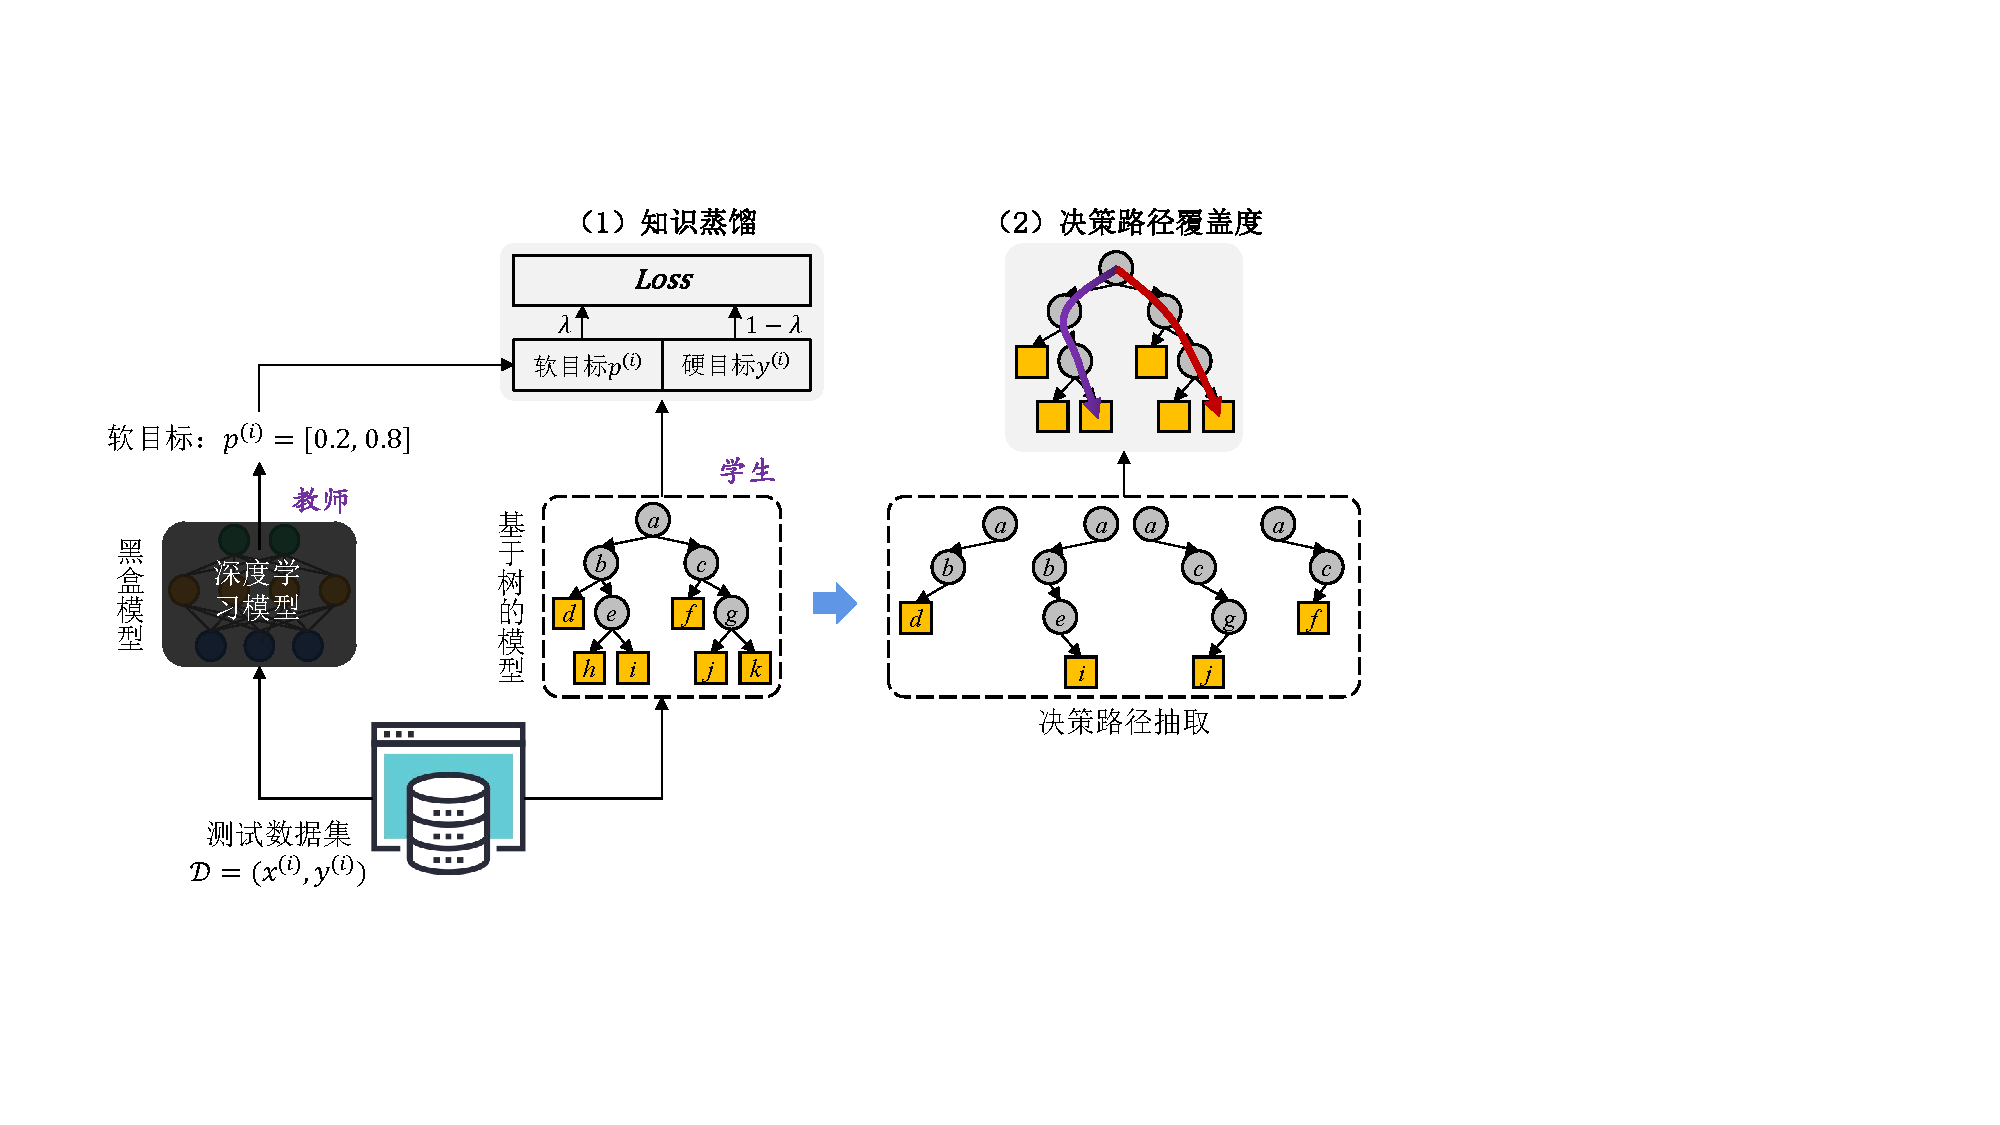
\includegraphics[width=0.9\textwidth]{ch3_2Btest.pdf}
        \end{center}
        \caption{基于决策行为模拟的黑盒测试研究方案}
        \label{fig:ch3:2Btest}
    \end{small}
\end{figure}

\textbf{本项目拟针对``学生''模型建立基于决策路径的覆盖性测试方法},知识蒸馏得到
的``学生''模型$\mathcal M_t$的预测行为非常接近原黑盒模型$\mathcal M$,针对
$\mathcal M_t$的覆盖度测试能比较准确地反映$\mathcal M$的泛化能力。首先,从基于树
的``学生''模型$\mathcal M_t$中抽取该模型对每个测试样本的决策路径,得到路径集合
$\mathcal P=\{t_1, t_2,\dots, t_l\}$,$l$表示路径数。然后,\textbf{本项目拟利用
统计方法建立基于决策路径的覆盖度指标},以评估测试用例集的充分性,其基本思想为对
树模型的决策路径覆盖度高的测试用例集具有良好的充分性,在此基础上,本项目拟计算决
策路径覆盖频率和正态分布的拟合程度来评估测试用例集的分布,可采用
Kolmogorov-Smirnov检验、D检验等方法,并结合正太性检验方法的拟合优度和决策路径的
覆盖度作为测试用例集充分性评价指标。此外,\textbf{本项目拟利用树模型的可解释性,
总结归纳模型错误行为的原因,指导训练数据集扩充和模型优化}。

\subsubsection{基于层次语义理解的白盒测试}\label{ch3_2}

本项目针对白盒测试的研究方案首先利用知识蒸馏技术,训练可解释的``学生''模型。以
\cref{fig:ch3:WBtestKD}为例,\textbf{本项目拟首先从给定的白盒模型中抽取其预测行
为},具体而言,本项目拟采线性判别分析(Linear Discriminative Analysis, LDA)抽取
各层样本表示的关键特征,同时可实现降维的效果,有效提高后续分析计算的效率,然后,
利用自底向上的层次聚类方法,对LDA得到的关键样本特征进行聚类,理清每一组神经网络
层的判别决策能力。本项目认为深度学习模型对输入的表示学习是一个从粗粒度到细粒度的
过程,因此,浅层表示(如第1组的输出)没有能力将样本分为最终指定的类别,仅能做到
粗粒度分类,但层次聚类算法会以打到最大类别数为目标,所以\textbf{本项目拟分析中间
层表示的整体分布,修改层次聚类的优化目标,或者在层次聚类之后,再合并相近的簇,以
准确反映中间层的决策语义}。

另一方面,\textbf{得到各组(层)的决策语义后,本项目拟改进知识蒸馏的方式,将各层
的决策语义融入``学生''模型的优化目标中},其主要思想如公式\eqref{eq:kd}所示:
\begin{equation}
    \mathcal{L} = \mathcal{L}_o + \beta\sum_{k=1}^L KL(p(f_s^k(\bm x_i)), p(g^k(y_i))) \,,
    \label{eq:kd}
\end{equation}
其中$\mathcal L_o$是``学生''模型原有的损失函数,$f_s^k(\bm x_i)$表示``学生''模型
第$k$层的表示向量,$g^k(y_i)$将数据标签$y_i$转换成第$k$层的语义标签,本项目拟用
KL散度来度量``学生''模型表示向量的分布是否和抽取的决策语义接近,作为损失函数的正
则项,引导``学生''模型训练。

\begin{figure}[htp]
    \begin{small}
        \begin{center}
            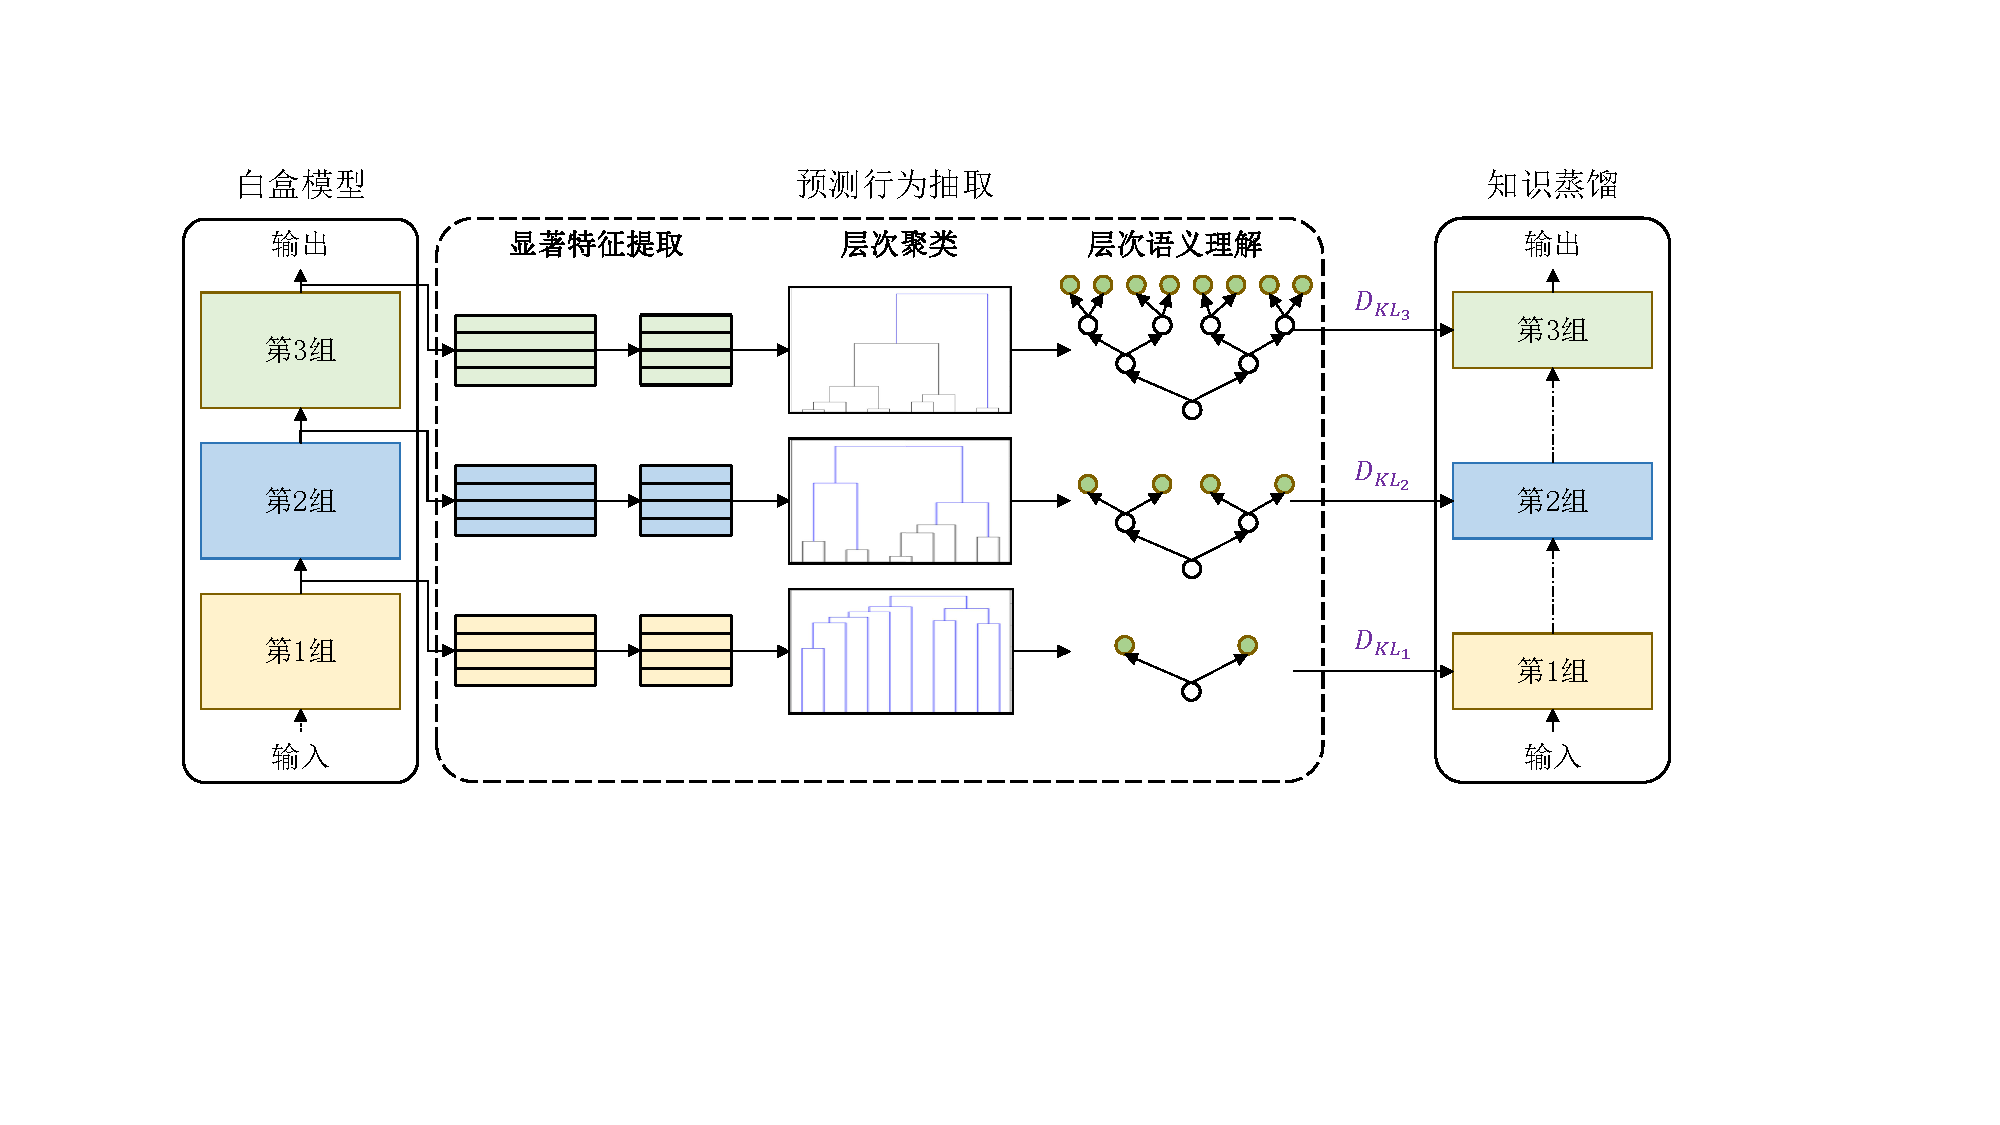
\includegraphics[width=0.95\textwidth]{ch3_WBtestKD.pdf}
        \end{center}
        \caption{基于层次语义理解的知识蒸馏研究方案}
        \label{fig:ch3:WBtestKD}
    \end{small}
\end{figure}

得到可解释的``学生''模型后,本项目拟基于该模型提出决策路径覆盖度测试指标。根据公
式\eqref{eq:kd},在测试阶段,容易得到各层输出所属的粗粒度类别,\textbf{如
\cref{fig:ch3:WBtest}所示,本项目拟分析测试用例集对该决策路径图的覆盖程度,用以
评估测试用例集的充分性,同时,可检测``学生''模型针对某样本的分类过程是否有异常决
策路径(图中虚线所示),以分析模型在不同测试用例上的泛化能力},具有异常决策路径
的测试用例可能是边界样本,很可能引发模型错误,是模型进一步优化提供重要参考。
\begin{figure}[htp]
    \begin{small}
        \begin{center}
            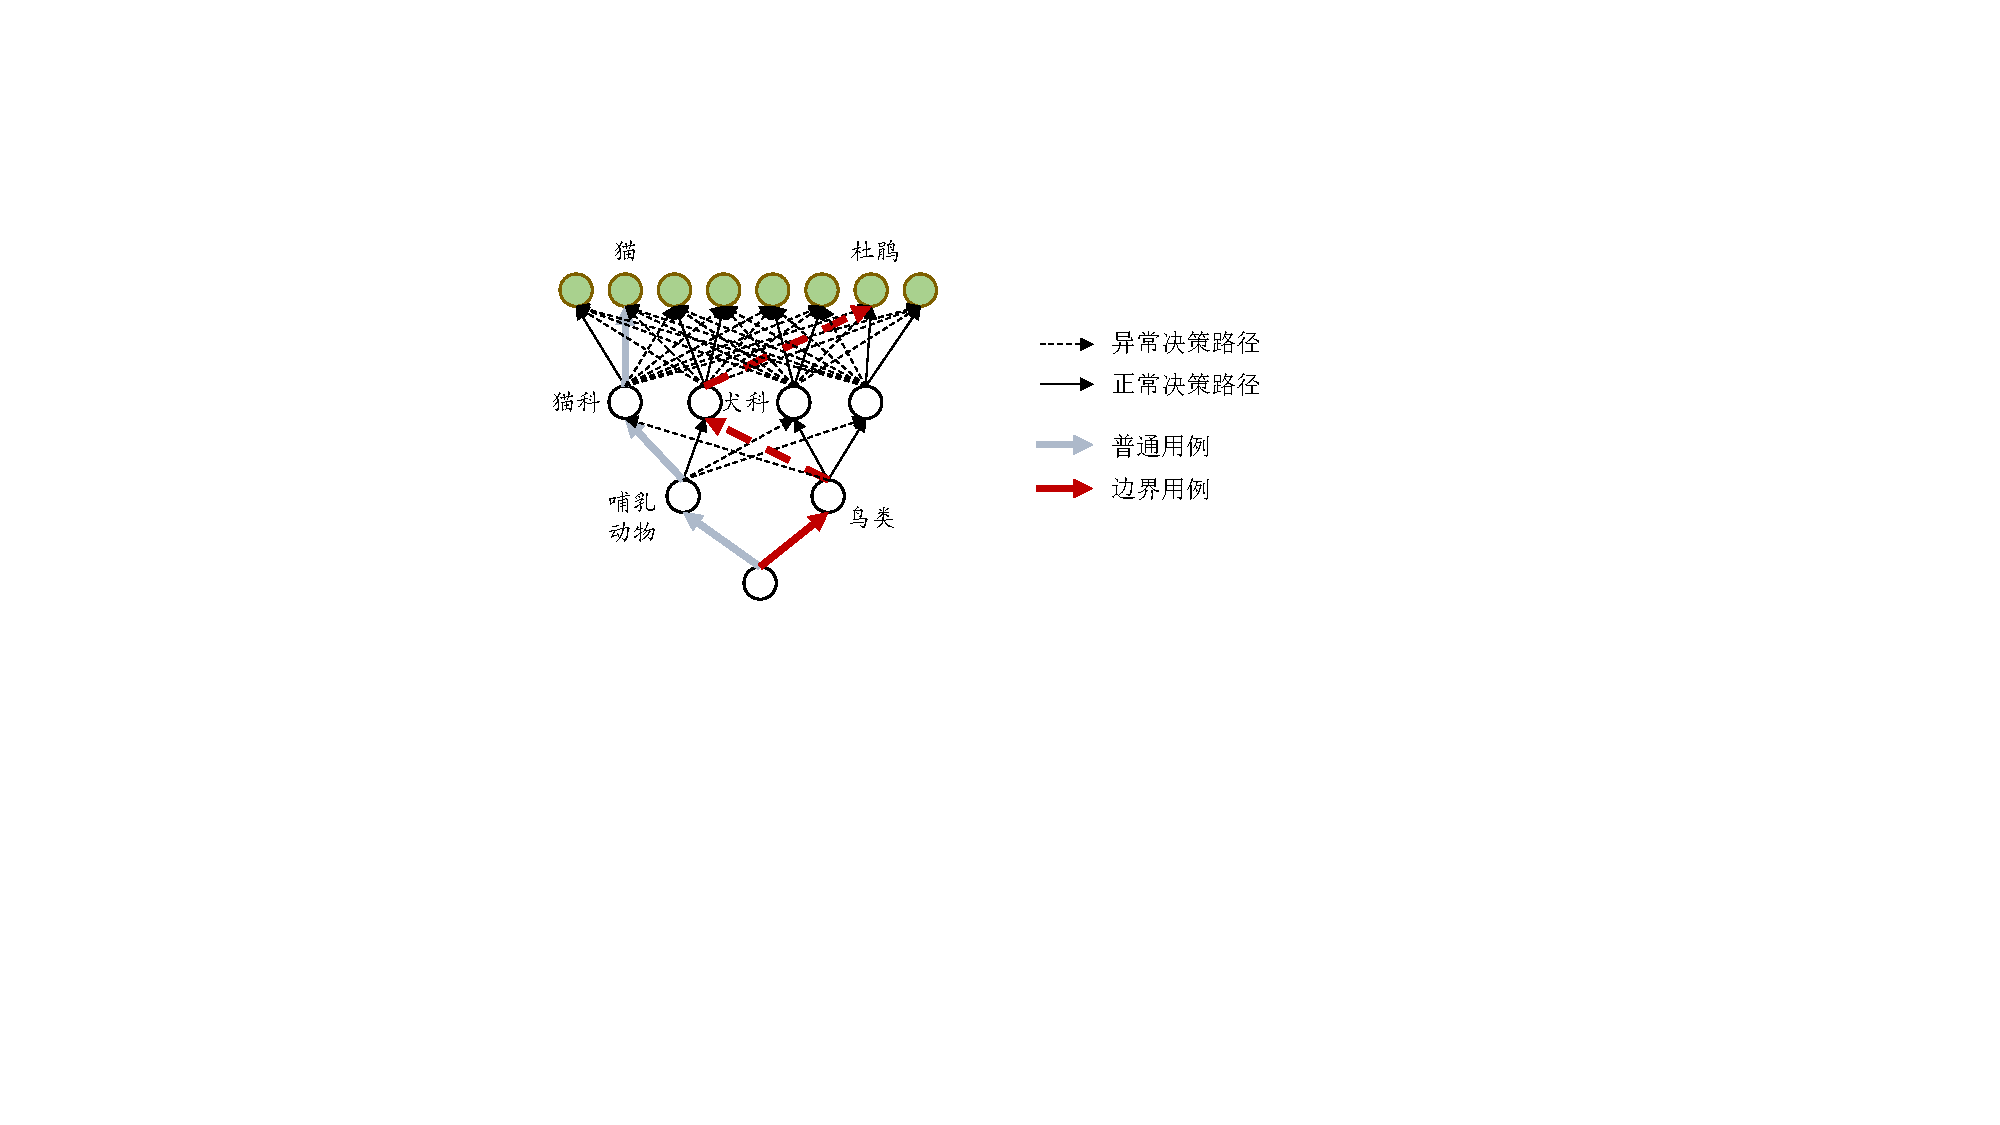
\includegraphics[width=0.65\textwidth]{ch3_WBtest.pdf}
        \end{center}
        \caption{基于可解释``学生''模型的覆盖度测试研究方案}
        \label{fig:ch3:WBtest}
    \end{small}
\end{figure}

\subsubsection{基于反馈偏置的自适应测试集生成}\label{ch3_3}

为了平衡测试集的规模和质量,针对给定大规模无标注数据,本项目拟在有限标注成本空间
内生成高质量测试集,尽可能模拟真实的测试数据分布,在\textbf{可控制规模内}生成具
有高代表性和检测能力的测试集,针对深度学习模型进行可解释测试。由于深度学习模型缺
乏可解释性且现有覆盖指标伸缩性差,本项目基于知识抽取方法模拟决策路径,将具有相同
决策路径的测试数据作为同类,采用\textbf{聚类分析和最大平均差异法}( Maximum Mean
Discrepancy,MMD)选取与大规模无标注测试数据具有近似决策路径分布的代表性数据作为
测试集,并反馈已选测试数据及其测试结果反馈,自适应选择测试数据。


\begin{figure}[htp]
    \begin{small}
        \begin{center}
            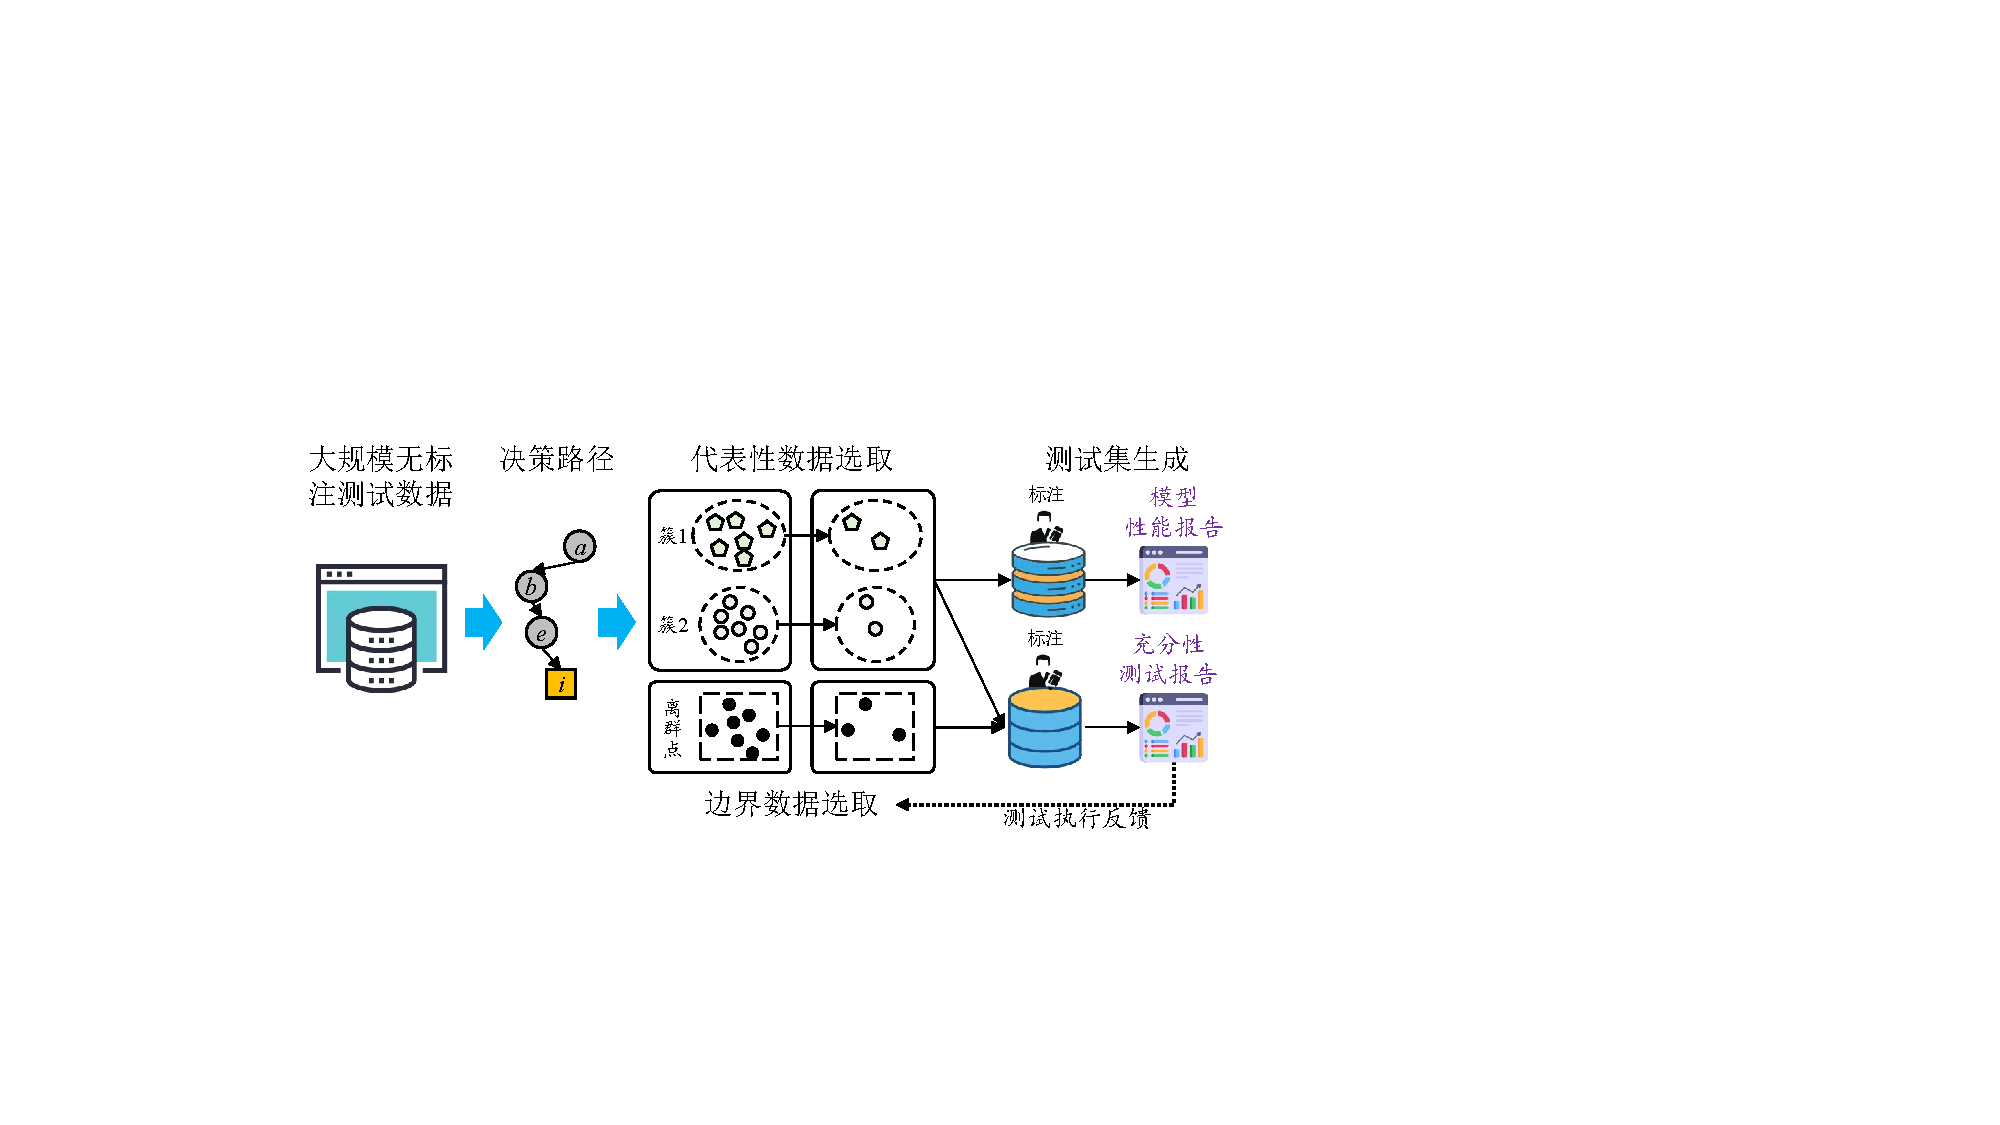
\includegraphics[width=0.85\textwidth]{ch3_TestSelection.pdf}
        \end{center}
        \caption{可解释预测模型(动态特征)研究方案}
        \label{fig:ch3:interpretability}
    \end{small}
\end{figure}

\cref{fig:ch3:interpretability}是本项目针对自适应测试集生成研究方案的示意图。首
先,为了测试的伸缩性和可解释性,采用知识蒸馏/知识回顾的方法抽取复杂神经网络的决
策路径,针对每个测试数据都获得其可解释性决策路径。以图中描述的模拟决策路径$t_i$
为例,每条决策路径对应$n_i$个无标注测试数据,视为一组。我们对每组测试数据进行聚
类分析,根据每组数据的规模将其聚为$k_i$类,然后利用最大平均差异的方法从每类测试
数据中选取$m$个测试数据,若该类数少于$m$个则全部选取,构成初始测试子集。最大差异
法可表示为以下公式:
\begin{equation}
    \begin{aligned}
        \operatorname{MMD}(\mathcal{F}, P, G)=\sup _{f \in \mathcal{F}}\left(\mathbb{E}_{X \sim P}[f(X)]-\mathbb{E}_{Y \sim G}[f(Y)]\right)
    \end{aligned}
\end{equation}
其中$\bm X= (\bm x_1, \bm x_2, \dots, \bm x_t)$为模型输入,$z$是隐变量,表示数据
特征的编号,$z \in {1,2,\dots, v}$,用于解释不同特征的重要性和时间关联性。
$I_{T_{1i}} \cdot \bm h_{1i}, I_{T_{2i}} \cdot \bm h_{2i}, \dots, I_{T_{ti}}
\cdot \bm h_{ti}$即为特征$i$时间维度的注意力,而$P(z=i|I_{F_1} \cdot \bm h_{t1},
I_{F_2} \cdot \bm h_{t2}, \dots, I_{F_v} \cdot \bm h_{tv})$则为特征$i$的全局重要
性。

反馈偏置为

{本项目拟从充分性测试和准确
评估模型两个测试目标来制定自适应反馈机制,将复杂神经网络抽象成可解释蒸馏模型,选
取与大规模无标注测试数据具有近似决策路径分布的代表性数据进行标注,为测试人员提供
全阶段的可解释测试方法}。

子集可经过可解释蒸馏模型得到所有测试数据的决策路径分布,具有相同决策路径的测试数
据为一组。根据每组测试数据规模大小,采用聚类分析将具有相同决策路径的测试数据分为
多个类簇,利用基于最大平均差异法为从每簇测试数据中选取固定总数的测试数据作为代表
性数据,得到与无标注数据集有近似决策路径分布的初始子集

\subsection{可行性分析}

\subsubsection{理论可行性}

本项目研究目标明确,研究内容清晰,研究方案和技术路线中所应用的方法和技术手段在业
界都有着成熟清晰的理论基础。申请人和项目组对这些关键技术和理论有着深入的了解和掌
握,近年来在人工智能、医疗数据分析等领域的高水平会议上发表了多篇论文。项目组前期
已经对本项目中提到的研究内容分别进行了详细的调研和分析,并在医疗特征表示学习、时
间序列插补等领域取得了初步成果。因此,从理论上说,本项目是可行的。

\subsubsection{技术可行性}

申请人前期调研了大量基于深度学习的电子医疗记录分析的研究工作(如
\ref{relatedwork}节所述),深度学习模型不仅能挖掘高维特征之间复杂的关系,同时能
有效处理数据中长时间依赖关系,非常适合电子医疗记录分析。利用深度学习技术解决电子
医疗记录预测性分析需要解决三个核心问题,即队列识别、EMR不规则性处理和模型的可解
释性,申请人之前的研究工作一直聚焦于电子医疗记录的分析,在医疗特征表示学习、多元
时序数据插补等方面已取得一定的研究成果,并在攻读博士期间与医生合作,参与过医疗分
析系统的开发,相关研发经验可作为本项目的研究基础。申请人所在项目组多年来一直活跃
在在大数据处理和分析、机器学习等领域,在相关领域有着丰富的研究经验和技术积累。同
时,在研究过程中,申请人与医疗机构建立了合作关系,积累了大量可用于实验的真实数据
集。因此,从技术上说,本项目是可行的。

\subsubsection{团队合理性}

项目组在大数据分析和人工智能领域具有一定的基础,积累了丰富的研究经验,在重要国际
会议上发表了多篇高水平论文,项目在信息系统和数据分析系统开发方面也有丰富的积累,
可为本项目可视化分析系统研发提供保障。项目组梯队完善,队伍具有凝聚力和创造力,项
目组成员每周定期讨论,有着良好的科研氛围,同时对本项目的研究内容具有浓厚的研究兴
趣。申请人与联合培养时的导师新加坡国立大学教授Beng Chin Ooi(黄铭钧)一直保持密
切联系,Ooi教授长期研究大数据管理与分析,是数据库和数据挖掘方面非常活跃的科学
家,可为本项目提供技术指导。

申请人与医疗机构和专家一直保持良好的合作关系,与北京大学医疗健康大数据国家研究院
张路霞教授合作研究慢性肾病患者病情进展,和天津市肿瘤医院合作研究肺癌患者治疗效果
评估,同时,申请人参与建设“南开大学-基准联合医学研究中心”,和广州基准医疗有限公
司合作研究基于多模态医疗数据的癌症早诊技术。这些合作单位和专家可为本项目提供专业
意见的反馈,保证研究内容符合医学常识和临床需求。综上所述,项目团队组成合理,能保
障本项目的顺利完成。